% @Author: YangZhou
% @Date:   2017-06-20 20:27:38
% @Last Modified by:   YangZhou
% @Last Modified time: 2017-06-28 17:35:13
\documentclass[%
 reprint,
 amsmath,amssymb,
 aps,
 prb,
]{revtex4-1}
\preprint{APS/123-QED}
\usepackage{graphicx}% Include figure filesxx
\usepackage{bm}% bold math
\newcommand{\angstrom}{\mbox{\normalfont\AA}}
\begin{document}
\title{Anisotropic in-plane thermal conductivity observed in multilayer silicene}
\author{Yang Zhou${}^{1,2}$}
\author{Chao-Yu Chen${}^{3}$}
\author{Zhi-Xin Guo${}^{3}$}
\email{zxguo08@hotmail.com}
\author{Shi-You Chen}
\author{Hong-Jun Xiang}
\author{Xin-Gao Gong${}^{1,2}$}
\email{xggong@fudan.edu.cn}
\affiliation{
  ${}^1$Key Laboratory for Computational Physical Science (Ministry of Education), State Key Laboratory of Surface Physics and Department of Physics, Fudan University, Shanghai 200433, China\\
  ${}^2$Collaborative Innovation Center of Advanced Microstructures, Nanjing 210093, Jiangsu, China\\
  ${}^3$Department of Physics, Xiangtan University, Xiangtan 411105, China
}
\begin{abstract}
  By means of non-equilibrium molecular dynamics simulation, we systematically study the thermal transportation properties of different types of multilayer silicon. It is found that the thermal transport properties of multilayer silicon structures have significant surface effect and size effect in thickness direction. Surface reconstruction affects heat transport very well , the thermal conductivity of bilayer silicon with different reconstruction can reach up to $11.6 W/mK$, and can be as low as $1.2 W/mK$ and the anisotropy can be as high as $57.3\%$.With the increase of the number of layers, the thermal conductivity of the zigzag direction changed little, but the thermal conductivity increased significantly in the armchair direction, and the anisotropy of thermal conductivity decreased which is due to the smaller affection in more layer structure. This work could be helpful in the field of heat management, thermoelectric applications involving silicon and other multilayer nano materials in the future.
  \begin{description}
    \item[Keywords]
          Thermal conductivity, multilayer silicon, surface reconstruction, anisotropy
  \end{description}
\end{abstract}

\maketitle

\section{INTRODUCTION}

With the development of the existing silicon based circuit industry, the requirements of its integration and miniaturization make a lot of research work focusing on the application of the new two-dimensional materials. The theory and experiments in the last 10 years show that some new two-dimensional materials have many novel and excellent physical properties due to their structure and size. For example, the single atom layer $MoS_2$ has a suitable band gap which makes its field effect transistor switching ratio as large as $10^8$ \cite{Li,Yu2014}. Black phosphorus (BP) with thicknesses of several atomic layer have extremely high electron / hole mobility ($1000cm^2/Vs$) and leakage current modulation rates ($10^4$ times of graphene) and the field effect transistor of it has great potential in the application of nano electronic devices\cite{RadisavljevicB2011}. Due to the high thermal conductivity and electron mobility of graphene, it has great potential applications in the field of nano circuits\cite{Chen2008,Balandin2008}. However, materials prepared in the practical application is often multilayer structure to a few nanometers. Previous studies have focused on the weak Van der Waals interaction (vdW), and there is no surface reconstruction. There have been lots of studies on the electronic and thermal transport properties for this kind of typical layered structure and hetero structures, such as graphene\cite{Lindsay2011,Ni2012,Wang2011}, $MoS_2$\cite{Liu2015}, black phosphorus\cite{Zhang2015,Peng2015,Jain2015} two-dimensional layered structure. The existing preparation technology such as mechanical stripping, molecular beam epitaxy has difficult to produce nano layered structure for the material with strong interaction between layers, and the research of this kind of super thin nano materials has been very scarce. Recently, it has been found that monolayer and multilayer silicon material can be grown on some metal substrates by molecular beam epitaxy\cite{Fleurence2012,Meng2013,Vogt2012,DePadova2013,Feng2012}. The progress of these experiments ignited the upsurge the two dimensional nanomaterials with strong interaction between layers. In contrast to vdW, the two layer nano materials, which are represented by multi-layer silicon, exhibit special surface reconstructions which are different from the bulk surface\cite{Fleurence2012,Meng2013,Feng2012,Guo2013} and its physical and chemical properties are also very unique\cite{Guo2013,Guo2015}, indicating that there is new physics in this kind of ultra-thin nano materials.

Silicon  is currently the only one system, from its monolayer to multilayer, and then to the bulk structure, that have been prepared by experiment. And it has rich and typical structure in the dimension of zero dimension, one dimension and three dimensions, which have laid a very good foundation for the study of two-dimensional scale multilayer silicon. The study of multilayer silicon is also helpful to understand the physical evolution of matter from low dimension to high dimension. In addition, the preparation process of silicon nano materials is mature and the raw materials are rich, and It has a broad application prospect in the fields of micro nano electronics, energy, information and other important fields in the future.

At present, research of thermal transport properties based on the silicon nano structure mainly includes silicon nanowires\cite{Hochbaum2008,Yang2010,Shi2009,Boukai2008}, silicene\cite{Pei2013,Ng2013,Xie2014,Zhang2014,Liu2014}, substrate supported silicene\cite{Wang2015,Zhang2015a}, silicon thin film and bulk structure\cite{Bodapati2006,Tang2013Thermal,Jeong2012Thermal,Liu2006Thermal,Wang2006Lattice}. Due to the quantum size effect in the thickness direction and surface reconstruction effect, silicon multilayer structure is expected to have lower thermal conductivity than the bulk and is more suitable for thermoelectric applications. However, the study on the properties of multilayer silicon thermal transport is still very rare, To this end, based on the first principles calculation of Guo\cite{Guo2015Structural}, we explored the thermal transport properties of the 2 to 10 layer silicon structure.

\section{COMPUTATIONAL DETAILS}

In this paper, based on the large scale parallel and efficient LAMMPS molecular dynamics software package\cite{Parks2007}, we study the thermal conductivity of multilayer silicon structure by using the non-equilibrium temperature gradient method. Because of the abundant silicon structure model, the phase reconstruction has attracted much attention. In order to well simulate the structures of different phase by MD, the latest Mod potential is chosen\cite{Kumagai2007Development}, which is able to reconstruct the silicon material elastic constants, the melting point and phase transition. Firstly, we use conjugate gradient method to optimize these structures. All structures are shown in FIG.\ref{fig:structures}.

\begin{figure}[b]
  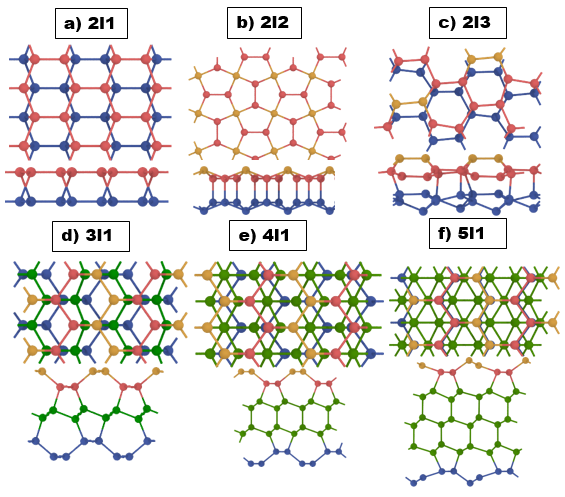
\includegraphics[width=0.48\textwidth]{images/structures}
  \caption{\label{fig:structures}  (color online) Some typical structure of multilayer silicon. Within which (a) to (e) are top view and side view of bilayer structures. (f) to (g) are side view of trilayer structures and (h) is that of four-layers. The buckling atoms on the top surface are labeled as yellow while the red atoms represent the others on the top surface. All the atoms on the bottom surface are labeled as blue. The blacks represent those that are inside the structure. The top view of the cells is shown in the last.}
\end{figure}

For convenience, we define the names of these structures as "nlxs", where n is a pure number, representing the number of layers, l represents layer, x distinguishes different structures (concrete 1, 2, 3 etc. ) and s indicates the type along the length direction with value of a (armchair) or z (zigzag). TABLE.\ref{tab:table1} lists the structure name, the minimum repeat cell periodicity, the binding energies, the first principle binding energies and the structural properties of the multilayer silicon. The Mod potential is constructed for different type of silicon structures by fitting its bond angle parameter to give correct melting point and elastic constants. It refers to the elastic properties predicted with first principle local density approximation (LDA) and the generalized gradient approximation (GGA). However, these first principle methods tend to overestimate the binding energy of materials and underestimate their equilibrium lattice constants. For this reason, the Mod potential is constructed referring the correction of the equilibrium bond length based on the experimental diamond structure and leads to smaller the binding energy than that predicted by the first principle method.

\begin{table*}
  \caption{\label{tab:table1}
    Symmetry of the structures, binding energy $E_c(eV/Si)$ and structure features}
  \begin{ruledtabular}
    \begin{tabular}{cccccccc}
      Name
           & Minimal period
           & Symmetry
           & $E_c$ in Guo
           & $E_c$ in MD
           & Buckling Feature                                                                       \\
      \hline
      2l1  & $1 \times 1$             & Cmme    & 5.000 & 4.145 & Smooth                            \\
      2l2  & $\sqrt{2}\times\sqrt{2}$ & C12/m1  & 4.991 & 4.204 & Large buckling and symmetric      \\
      2l3  & $2 \times 2$             & C12/m1  & 5.063 & 4.257 & Large buckling and tilt symmetric \\
      2lh  & $2 \times 2$             & P1      & 5.073 & 4.216 & Large buckling                    \\
      2lr3 & $\sqrt{3}\times\sqrt{3}$ & P1      & -     & 4.225 & Small buckling and symmetric      \\
      3l1  & $2 \times 1$             & P121/m1 & 5.138 & 4.337 & -                                 \\
      3l2  & $2 \times 1$             & P1      & 5.135 & 4.298 & -                                 \\
      4l1  & $2 \times 1$             & P1      & 5.225 & 4.368 & -                                 \\
      2l2  & $\sqrt{2}\times\sqrt{2}$ & C12/m1  & 4.991 & 4.204 & Large buckling and symmetric      \\
      2l3  & $2 \times 2$             & C12/m1  & 5.063 & 4.257 & Large buckling and tilt symmetric \\
      2lh  & $2 \times 2$             & P1      & 5.073 & 4.216 & Large buckling                    \\
      2lr3 & $\sqrt{3}\times\sqrt{3}$ & P1      & -     & 4.225 & Small buckling and symmetric      \\
      3l1  & $2 \times 1$             & P121/m1 & 5.138 & 4.337 & -                                 \\
      3l2  & $2 \times 1$             & P1      & 5.135 & 4.298 & -                                 \\
      4l1  & $2 \times 1$             & P1      & 5.225 & 4.368 & -                                 \\
    \end{tabular}
  \end{ruledtabular}

\end{table*}

From TABLE.\ref{tab:table1}, by comparing the binding energy of the first principles calculation of Guo is with that of MD, and from the point of view of stacking, the double layer of silicon is found more likely to form a monolayer of small and medium buckling slip stacking structure. The simulation is doing by velocity Verlet integral algorithm with the timestep to be $1 fs$. The length of the system in the x direction is $10 - 100nm$, the transverse direction y is in periodic boundary condition with its simulated width to be 5 nm, and free boundary condition is applied in z direction. At the same time the outermost two ends of the x direction are fixed, close to witch a 3nm with Nose-Hoover bath is applied. The left and right ends of the temperature control at $310K$ and $290K$. The simulation is carried out by NVT for $0.4ns$, then control the temperature gradient for $10 ns$, and finally we statistics the data of the last $10ns$. By Fourier's law, the relationship between thermal conductivity and heat flux is

\begin{equation}
  \kappa = \frac{ J_x}{ \nabla T \cdot S} \label{eq_nemd}
\end{equation}

where $\kappa$ stands for thermal conductivity, $J_x$ , $\nabla T=(T_L-T_R)/L_x$ is the average heat flux and temperature gradient along x direction respectively. $T_L$, $T_R$ and $L_x$ means the temperature of the two ends and the sample length between the heat baths. $S=W \cdot nd$ is the total cross area, where W,n,d is the size in the y direction, the layer number and the thickness of each layer. According to the previous studies, we choose Si (111) layer spacing of $3.14 \angstrom$ as the thickness of each layer.



\section{RESULTS AND DISCCUSION}

We firstly investigate the effect of surface reconstruction on thermal conductivity. 5 kinds of silicon structures of armchair and zigzag were selected to study. The relationship between the thermal conductivity and the length of bilayer silicon in different directions is shown in FIG.\ref{fig:2l_length}. the thermal conductivity of 2l1 structure increases with the length the most significantly, followed by the 2l3 structure and 2lr3 structure, while the least significant is the structure of 2l2 and 2lh. In addition, the structure with the thermal conductivity increasing significantly with the length is obviously anisotropy, different from single layer silicon and bulk silicon, who tend to be isotropic. In the aspect of structural, smooth 2l1 is most favorable for heat conduction, while 2l2 structure whose surface is made of a highly symmetrical and highly buckling pentacyclic ring "bird cage" is most unfavorable for thermal conductivity but suitable for thermoelectric materials. And the edges of the two directions are similar in shape, leading to small difference of heat transport.

\begin{figure}[b]
  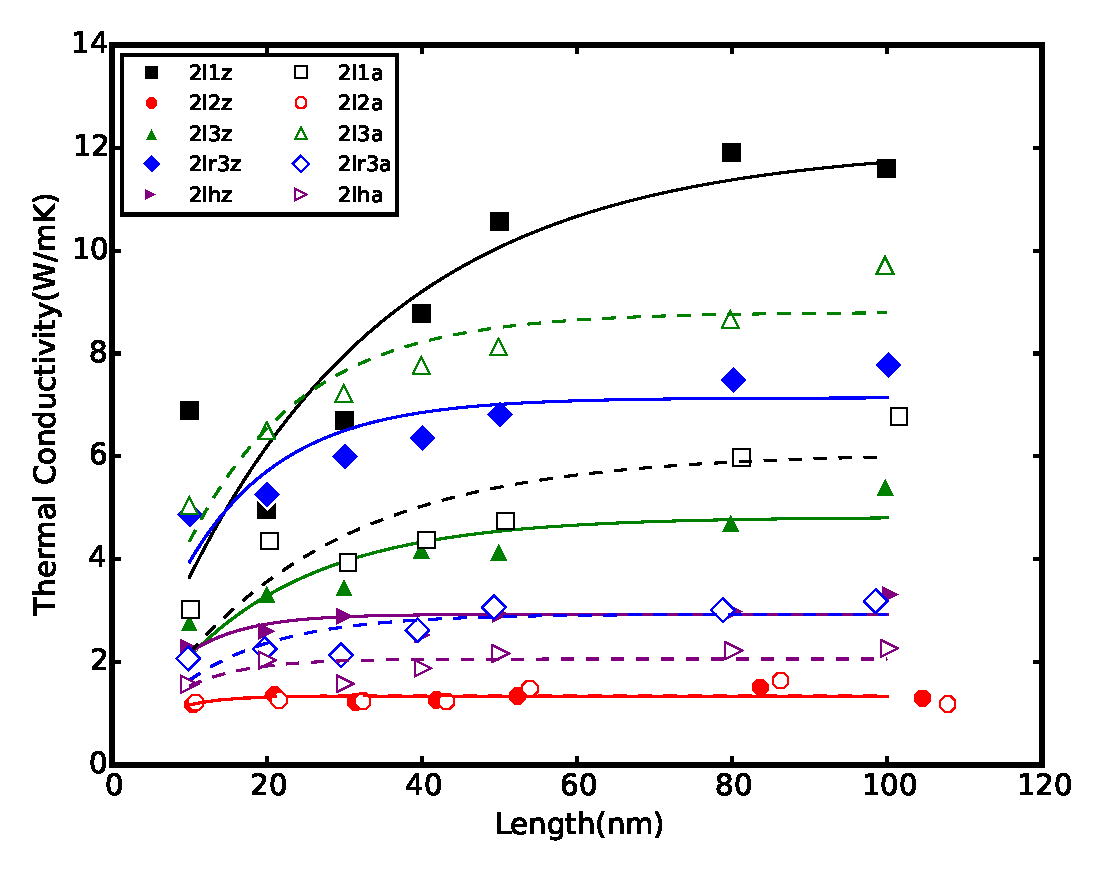
\includegraphics[width=0.48\textwidth]{images/2l_length}
  \caption{\label{fig:2l_length} (color online) The thermal conductivity dependence on length for five types of bilayer silicon. The scatters are the results of MD simulations while the lines are fitted with Eq.\ref{eq_nemd}. The letter z/a in the legend mean the transport direction is zigzag/armchair.}
\end{figure}

\begin{figure}[b]
  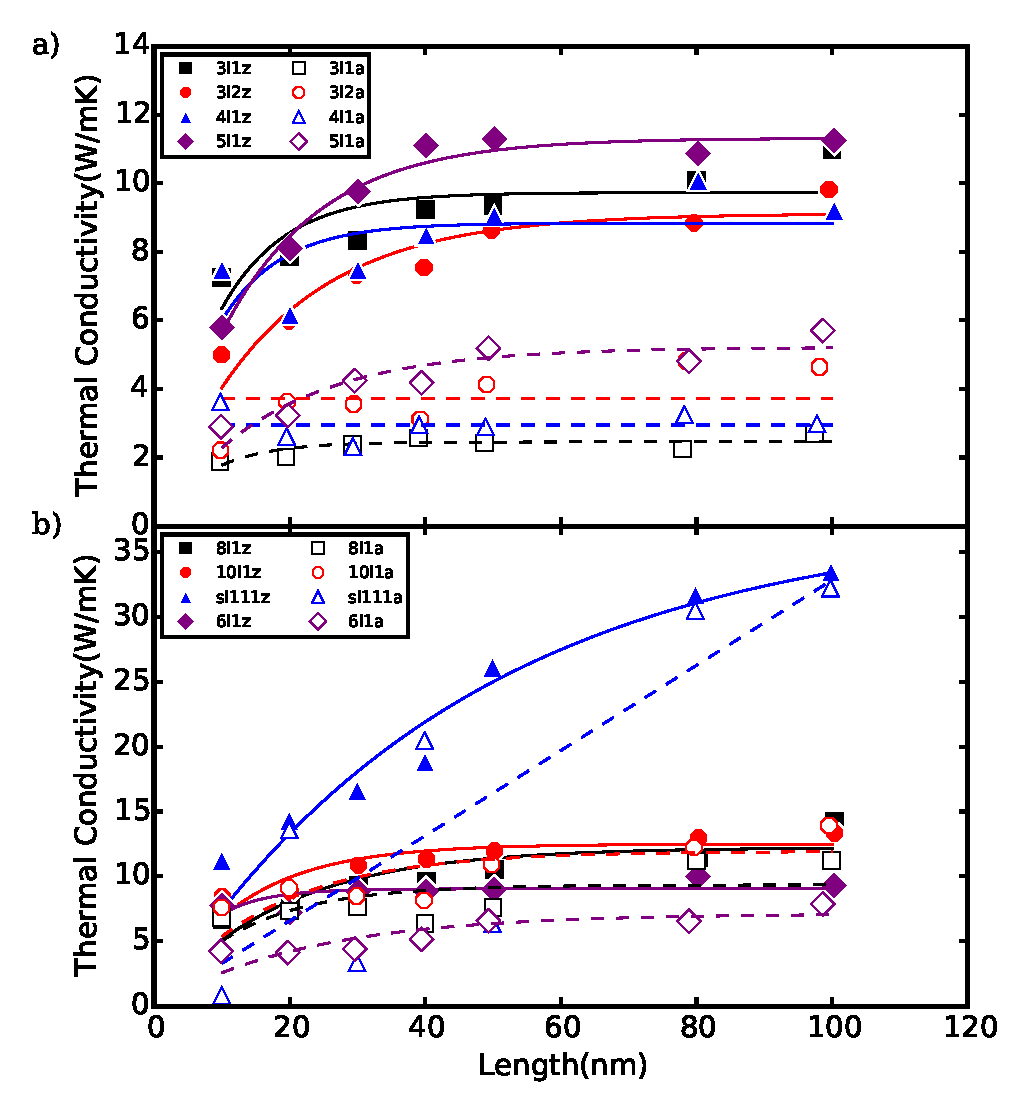
\includegraphics[width=0.48\textwidth]{images/vl_length}
  \caption{\label{fig:vl_length}(color online) The dependence on length of thermal conductivity for silicon with variable layers.}
\end{figure}

When the length of the silicon is smaller than the mean free path of the phonon, the ballistic transport properties of the phonon are obvious. When the length is larger than the mean free path of the phonon, the phonon scattering transport characteristics are obvious. The empirical formula of the John A. Thomas\cite{Thomas2010} can be used to characterize the thermal conductivity of the phonon transport from ballistic to scattering region, at the same time accurately obtaining thermal conductivity of the infinite long nano materials. Using this formula, we obtain the thermal conductivity of infinitely long multilayer silicon
\begin{equation}
  \kappa = \kappa_\infty (1-e^{-\frac{L}{L_c}})
\end{equation}

where $\kappa_\infty$ is the fitted full scattering thermal conductance. $L_c$ is the transition length from the ballistic transportation to the scattering transportation. The value $ \chi=|\kappa_{z,\infty}-\kappa_{a,\infty} |/max⁡(\kappa_{z,\infty}-\kappa_{a,\infty} ) \times 100 \%$ is used to measure the thermal conductivity difference in different directions, where $ \kappa_{z,\infty} (\kappa_{a,\infty})$ stands for the full scattering thermal conductivity (infinite thermal conductivity) in the zigzag (armchair) direction. And is $ max⁡(\kappa_{z,\infty}-\kappa_{a,\infty} ) $ the maximum value of thermal conductivity in the two directions.

The thermal conductivity and anisotropy of multilayer silicon is shown in TABLE.\ref{tab:table2}. It can be seen from the table that the thermal conductivity of the bilayer silicon can reach up to 11.6 W/mK (2l1 structure). In addition, the 2lr3 with small top and bottom buckling possesses the most anisotropy, which can reach 57.3\%. The smallest is 2l2 and 2lh (20\%). The above results show that surface reconstruction has a significant effect on the thermal transport properties of multilayer silicon. The smooth surface is favorable for heat conduction, while the rough surface can greatly suppress the heat conduction. Meanwhile, the anisotropy of the surface structure leads to the significant anisotropy of the thermal conductivity.

\begin{table*}
  \caption{\label{tab:table2}
    The thermal conductivity and anisotropic ratio of different multi-layer silicene.Along with the average heat capacity ($kJ/m^3/K$) of zigzag direction and armchair direction.}
  \begin{ruledtabular}
    \begin{tabular}{cccccccccccc}
            & $\kappa_{z,\infty}$
            & $\kappa_{a,\infty}$
            & $\chi$
            & $Cv_{z}$
            & $Cv_{a}$
            &
            & $\kappa_{z,\infty}$
            & $\kappa_{a,\infty}$
            & $\chi$
            & $Cv_{z}$
            & $Cv_{a}$                                                                                              \\
      \hline
      2l1   & 11.6                & 6.5  & 43.9\% & 165.8 & 166.7 & 2l2      & 1.5  & 1.2  & 20.0\% & 38.44 & 38.44 \\
      2l3   & 5.0                 & 9.7  & 48.5\% & 23.38 & 23.38 & 2lr3     & 8.2  & 3.5  & 57.3\% & 10.15 & 10.15 \\
      2lh   & 2.0                 & 2.5  & 20.0\% & 22.42 & 22.42 & 3l1      & 11.5 & 2.9  & 74.8\% & 52.22 & 52.46 \\
      3l2   & 10.2                & 5.2  & 49.0\% & 55.56 & 55.84 & 4l1      & 10.2 & 3.4  & 66.7\% & 37.71 & 37.89 \\
      5l1   & 11.7                & 5.7  & 51.3\% & 29.17 & 29.32 & 6l1      & 10.3 & 7.8  & 24.3\% & 23.73 & 23.86 \\
      8l1   & 13.2                & 14.9 & 11.4\% & 17.26 & 17.36 & 10l1     & 13.3 & 13.5 & 1.5\%  & -     & -     \\
      Si111 & 33.6                & 34.7 & 3.2\%  & -     & -     & Silicene & 11.4 & 11.6 & 1.7\%  & 606.4 & 613.4 \\
    \end{tabular}
  \end{ruledtabular}
\end{table*}

The influence of thickness change on the thermal transport properties was then investigated. Here we study mainly on multilayer silicon structure with 3-10 layers, whose  surface has typical Si (111) $2 \times 1$ surface reconstruction. In order to compare, we also calculated the thermal conductivity of Si on its (111) surface and the thermal conductivity of the monolayer. The magnitude of the anisotropy is also shown in TABLE.\ref{tab:table2}. From the FIG.\ref{fig:vl_length}(a), in the case of the medium thickness of the 3 - 6 layers, the anisotropy of the multilayer silicon with zigzag type is higher than that of armchair. And with the increase of the number of layers, the anisotropy decreases gradually. The reason is that the zigzag direction of the multilayer silicon surface is composed of a smooth zigzag atomic chain (as shown in FIG.\ref{fig:structures}). Compared with the bulk silicon structure, the heat conduction along the zigzag direction has no obvious effect on the heat flow. While along the armchair direction, the fluctuation of multilayer silicon surface is very large, the same is its obvious affection on heat flow. This difference is mainly caused by the surface reconstruction effect, and will decrease with the increase of the thickness of the silicon. In order to predict the relationship between the thermal conductivity and the thickness, we calculated the thermal conductivity of the 8-10 layers silicene with the $2 \times 1$ surface reconstruction. In order to compare, the thermal conductivity of the bulk Si (111) surface with no surface reconstruction (9 layers) and the thermal conductivity of the monolayer were calculated. As shown in TABLE.\ref{tab:table2}, with the increase of thickness, the anisotropy decreases gradually. When the thickness is up to 10 layers, the anisotropy of the thermal transport of multilayer silicon can be neglected (only about 1.5\%), which is consistent with the results of bulk silicon and single silicon. On the other hand, as shown in FIG.\ref{fig:vl_length}(b), at the same thickness, in the case of shorter length (10 - 50nm), the anisotropy is obvious. When the length is about 100nm, the anisotropy difference becomes very small, and the size effect of the thermal conductivity anisotropy is obvious. This is essentially due to the difference in the out-of-plane acoustic branch (LA), the transverse acoustic branch (TA), and the vertical plane acoustic phonon (ZA) of the multilayer silicon structures along different directions. However, with the increase of length, the ballistic transport is gradually saturated, and the difference of the heat transfer caused by the umklapp process is gradually reduced.

\begin{figure}[b]
  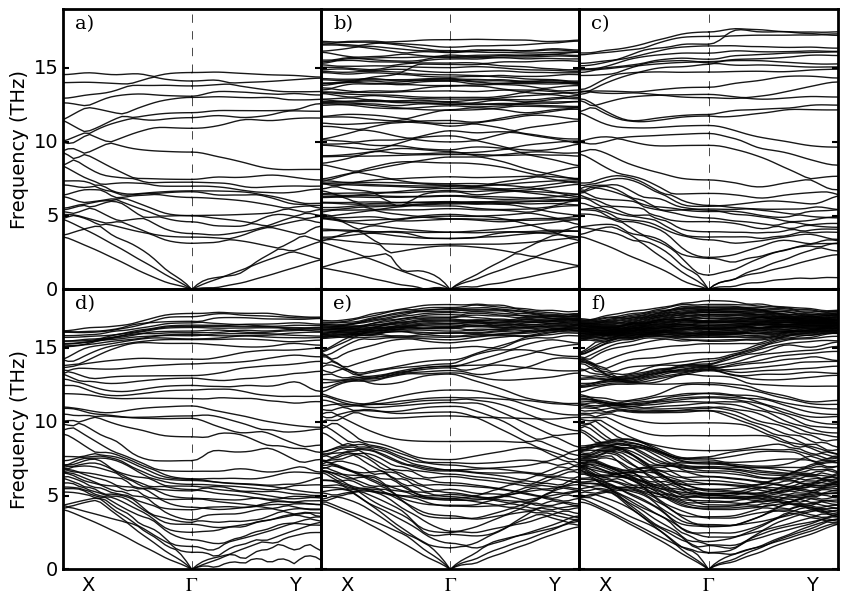
\includegraphics[width=0.48\textwidth]{images/bands}
  \caption{\label{fig:bands}(color online) The phonon dispersion of multilayer silicon along high-symmetry points. (a)2l1 and (b) 2l2 are bilayer structure (c) 3l1 is trilayer structure, (d) 4l1 is four-layer structure and (e) 6l1 width six layers, (f)10l1 with ten layers.}
\end{figure}

In order to understand the relationship between the thermal conductivity and the length of the different structures and different layers, we calculated the phonon spectra of several typical structures. The $10 \times  10  \times  1$ multilayer structure is chosen. The selected high symmetry points are $\Gamma(0.0, 0.0, 0.0)$, $X(0.5, 0.0, 0.0)$,  $Y(0.0, 0.5, 0.0)$, Take points along $ X \rightarrow \Gamma \rightarrow Y$ as shown in FIG.\ref{fig:bands}.According to the supercell structure, the zigzag boundary corresponds to $ \Gamma \rightarrow X$ direction in the dispersion, and the armchair boundary corresponds to $\Gamma\rightarrow Y$ direction. According to the relationship between the phonon spectrum and heat conduction, in the two-dimensional nano system, the acoustic phonon plays a major role in heat transport. There are a total of 3 acoustic branches, including the LA mode along the transmission direction, TA along the transverse and ZA mode along the perpendicular direction. FIG.\ref{fig:bands}(a) and (b) corresponds to the calculated spectra of the bilayer structure 2l1 and 2l2. The group velocity of $\Gamma\rightarrow X$ acoustic branch in 2l1 is obviously larger than that of $\Gamma\rightarrow Y$, making zigzag direction more heat conducive , which also verifies the difference between 2l1z and 2l1a thermal conductivity and anisotropy. Accordingly, the three phonons in the two direction is almost the same as that in the 2l2, so the 2l2z and 2l2a are the least anisotropic structures with surface reconstruction. Comparing the two graphs, it can be found that all the group velocities of three phonons of 2l2 decrease. At the same time, the low frequency optical branch has the trend of moving down and couple with acoustic ones, which makes it less heat conducive, so that the 2l2 heat transport changes little with the length. The figure (c) (d) (e) is the dispersion of 3l1, 4l1, 6l1 $2 \times 1$ structure, all of whose three phonon group velocity are larger along zigzag than armchair. With the increase of layers, the optical branch participation gradually gathered in the high frequency area ($>15THz$), having almost no contribution to thermal conductivity while the vibration mode of the low frequency ($<5THz$) region is almost unchanged. On the other hand, with the increase of thickness, the acoustic velocity of armchair direction increases gradually, which prompts the decrease of anisotropic in multilayer silicon with the increase of layer number. Compared with phonon spectrum of the 6-layer structure(e), the difference between the 10 layers (f) is mainly the contribution of more atoms in the middle and high frequency ($>5THz$) region, which has little effect on the thermal conductivity.

The thermal conductivity tensor could be calculated with

\begin{equation}
  \kappa^{\alpha\beta} = \sum_{k \sigma}{c_{k \sigma}v^{\alpha}_{k \sigma}v^{\beta}_{k \sigma}\tau_{k \sigma}} \label{eq:kappasum}
\end{equation}

Where $c_{k \sigma}$ means heat capacity of phonon mode $k \sigma$, $v^{\alpha}$ present for mode group velocity and $\tau_{k \sigma}$ is phonon lifetime. The anisotropy could derive from these factors and it's worth finding the most important ones.

Heat capacity has large influence between the structures but has no contribution to anisotropy. We select all the phonons along  $\Gamma\rightarrow X$ , calculate each of their heat capacity with

\begin{equation}
  c_{k \sigma}=\frac{\hbar \omega_{k \sigma} }{V} \frac{\partial f(\omega_{k \sigma},T)}{\partial T}
\end{equation}

Where $ f(\omega,T)=1/(exp(\frac{\hbar \omega}{k_b T})-1)$ is Bose-Einstein distribution function. The values are averaged to get $Cv_z$ while those of phonons along $\Gamma\rightarrow Y$ are called $Cv_a$. The average heat capacity of the structures are shown in Table.\ref{tab:table2} . Large difference could be found between the $Cv$ of the structures. The lowest value is $10.15 kJ/m^3/K$ of 2lr while the highest value of Silicene could reach $606.4 kJ/m^3/K$, and this could lead to large difference between their thermal conductivity. There's no obvious trends when the layer increases but Silicene and 2l1 have pretty large value than the others and this has some relation to their low thickness.  Almost no difference could be found in the value along zigzag direction and armchair direction, even if $\omega_{k \sigma}$ has large deviation between the direction as shown in Fig.\ref{fig:bands}. This is due to the insensitivity of heat capacity to frequency when the frequency is low and the value is ignorable when frequency is relatively high. That means when considering only acoustic phonons the heat capacity is close to constant.


\begin{figure}[b]
  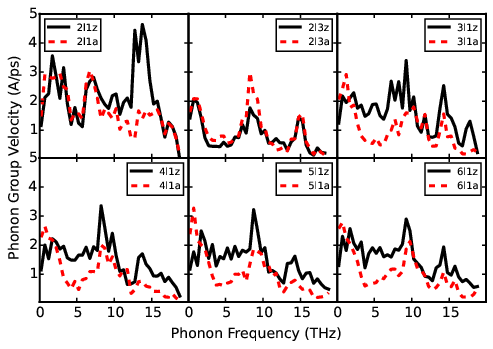
\includegraphics[width=0.48\textwidth]{images/gv}{}
  \caption{\label{fig:gv} (color online)Group Velocity.}
\end{figure}

The anisotropy of phonon velocity has little contribution for the anisotropy of the thermal conductivity. FIG.\ref{fig:gv} showes the group velocity along both zigzag and armchair direction for all the structures. The group velocity  along the two directions of  2 layers silicene ( include silicene) are exactly the same except for that of 2lr3 structure whose low frequency group velocities are highly anisotropic. Group velocity for the others are all highly anisotropic and it's obvious that the group velocity of armchair direction are all large than that of zigzag. The relation between the group velocity of both direction are contrast with that of the thermal conductivity, which indicate that the main effect of anistropy is not from group velocity but the scatter rate origin from anharmonic effects.

\begin{figure}[b]
  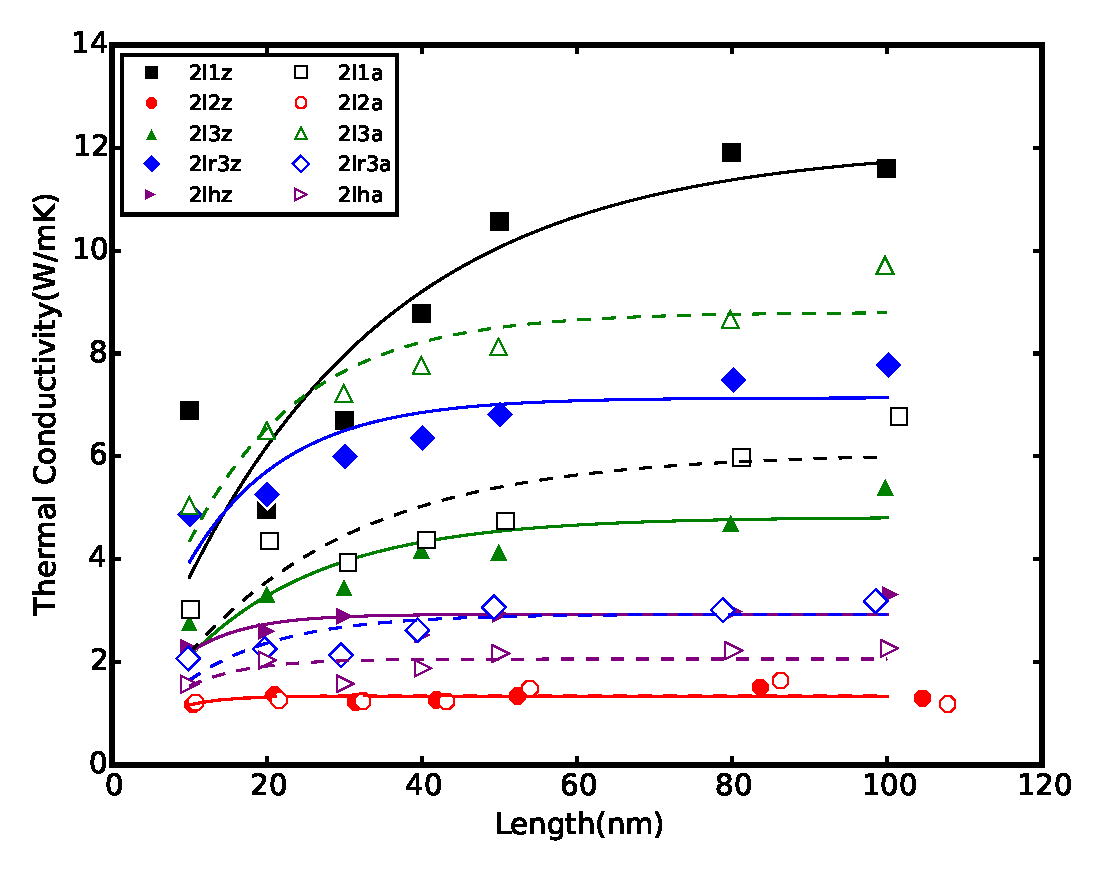
\includegraphics[width=0.48\textwidth]{images/pr_direction}
  \caption{\label{fig:pr_direction} (color online) The participation ratio.}
\end{figure}

The different localization situation  along each direction determines the anisotroy of group velocity  along that direction. To qualitatively measure the physical mechanism of phonon localization we carried out a vibrational eigenmode analysis. Mode localization can be quantitatively characterized by the phonon participation ratio $P_{k\sigma}$  \cite{Allen1999}for each eigen-mode $k\sigma$ as

\begin{equation}
  P_{k\sigma}= \frac{1}{N \sum_{i}
    {(\sum_\alpha{\epsilon^{i\alpha}_{k\sigma}
        \epsilon^{*i\alpha}_{k\sigma}})^2}}
\end{equation}

where N is the atom number and $\epsilon^{i\alpha}_{k\sigma}$ is the eigenvector component of mode $k\sigma$ for the i-th atom and $\alpha$ direction. The value of participation ratio is between 0 and 1 which measures the fraction of atoms participating a given phonon mode. If the mode is localized then its trends with N is O(1/N) while delocalized modes with O(1).

The anisotropy of phonon participation ratio has low contribution to anicotropy of thermal conductivity of low layers but have large contribution to that of large layer structures. In previous work we have proven that phonon participation ratio has obvious correlation with ballisic thermal transpotation in two dimentional materials\cite{Zhou2016}. Fig.\ref{fig:pr_direction} shows average phonon participation ratio for each eigenmode $k\sigma$ in various structures. The participation ratio of similar frequency has large difference and we select the phonons along zigzag direction and  average their participation ratio to obtain the solid black curve in Fig.\ref{fig:pr_direction} while the same is done to obtain the dash red curve for armchair direction. All the phonons of Silicene , 2l1 and some low frequency phonons of 2l2 exibit delocalized nature,suggesting that every phonon has been participated by all the atoms, which is due to the perfect bonding of them without dangling bonds. Different surface situation affects the localization a a lot. 2l3 and 2lr3 exhibit large localization and anisotropy even for very low phonons, this is due to their unique surface where the buckling atoms form parallel lines, between them existing large distance,see Fig.\ref{fig:structures}. With the increasement of thickness, low frequency region remain delocalized while the participation ratio of intermediate frequency  decreases. For 6l1 the average participation ratio could drop down to around 0.4, and that of 8l1 even to 0.3. But the absolute number of atoms that participate in the mode $P_{k\sigma} \cdot N$ does not decrease and the number of transmission chanels in fact increase so thermal conductivity increase.

\begin{figure}[b]
  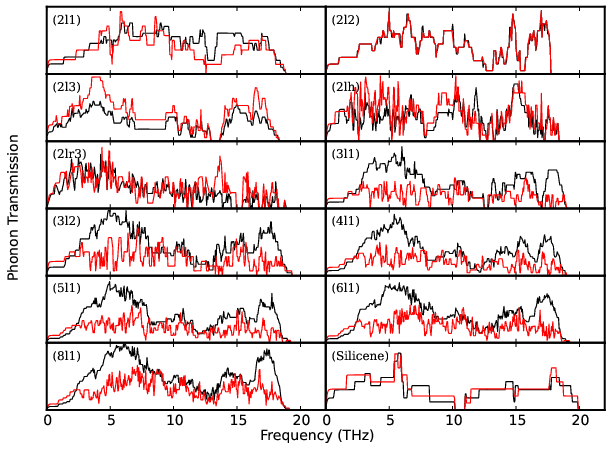
\includegraphics[width=0.48\textwidth]{images/transmission}
  \caption{\label{fig:transmission} (color online)The anisotropic transmission function of the structures. The structure identifiers are labeled at top-left of each subplot. the transmission along zigzag direction is ploted as black curve while that of armchair direction is filled. The y range of each subplot is normalized to the max value within the graph.}
\end{figure}

To quatitily study the number of transmission channels we use Non-Equalibrium Green Function (NEGF)\cite{Mingo2003} to calculate the transmission function of the struction along zigzag and armchair direction.
The transmission function can be expressed as
\begin{equation}
  \begin{split}
    \Theta(\omega)= Tr(
    \mathbf{\widetilde{k}}_{a\alpha}
    Im(\mathbf{g}_{\alpha\alpha})
    \mathbf{\widetilde{k}}_{\alpha a}
    \mathbf{G}_{a b}^*\\
    \mathbf{\widetilde{k}}_{b\beta}
    Im(\mathbf{g}_{\beta\beta})
    \mathbf{\widetilde{k}}_{\beta b}
    \mathbf{G}_{b a}
    )
  \end{split}
\end{equation}
where $\mathbf{\widetilde{k}}_{a\alpha}$,$\mathbf{\widetilde{k}}_{\alpha a}$ represents for the interaction between left lead and center region and its transposition,  $\mathbf{\widetilde{k}}_{b\beta}$,$\mathbf{\widetilde{k}}_{\beta b}$ the interaction between center and right lead. $\mathbf{g}$ and $\mathbf{G}$ the retarded Green's function of the leads and center rigion.$Tr$ and $Im$ means trace and imaginary function. Transmission function represents for the number of channels of a given frenquency. The more chanels means larger capability of thermal transportation. The value is substracted by the cross area of the transportation direction to eliminate the effect of lattice constants.

FIG.\ref{fig:transmission} shows the phonon transmission function along both zigzag and armchair directions. The y-axis value of each panel is not the same so the transmission is given here only to explain the anisotropy of each strcutre. The steps in the curves are  characterisic of perfection of the structure. Defects like isotope or grain boundary could lead to disapearance of these step.The transmission of Silicene and 2l1 are perfectly stepwise because of the perfect bonding and the absence of disorder.

Similar to the situation of participation ratio, transmission of both directions of Silicene,2l1 are close.Especially that of 2l2 are exactly the same, which is due to the structure symmetry of it.The anistropy of the transmission are clearly found in other structure,such as 2l3,3l1,3l2,4l1, where transmissioin of 2l3 is larger in armchair direction than zigzag,while the others has smaller value in armchair. This trends is quite consist with that of the thermal conducivity so transmission indeed has large effection on the difference of thermal conductivity. The transmission along zigzag direction has a large peak at around 5THz in the structure 3l1,3l2,4l1,5l1,6l1,8l1,while along armchair direction the peak vanish and this may contribute a lot to the anisotropy of the thermal transportation.

\begin{figure}[b]
  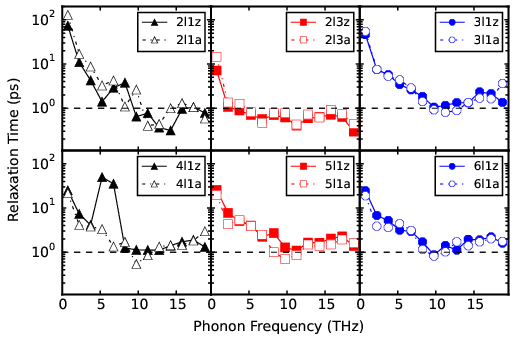
\includegraphics[width=0.48\textwidth]{images/tau}
  \caption{\label{fig:tau} (color online)Lifetime.}
\end{figure}

The ballistic contribution of long wave phonons clearly indicate that localization dominant the anitropy of the structures, but more contribution should origin from phonon scattering. We only considering three-phonon scattering,which consist of two types of scattering process, one of them is two phonons vanish and one phonon created and the other type is one phonon transform to two phonons. Both of them are possible to have result phonons with q point outside Brioulls boundry, and it must be fold back to Briulls zone to make the result physcical. So this process is called Umpack process( U process). And of cause there exist the situation that none of the three q points outside the Brioulls boundry, and the summation of the momentum conserves ( $q''=q+-q'$), which is called Normal process (N process) or momentum conservation process. If there's no U process the thermal conductivity could be as large as possible, so this process give the dominent contribution to thermal resistance. The phonon scattering rate could be obtained by Fermi-golden rule 

\begin{equation}
\end{equation}

considering only the relaxation time approxmition(RTA). We then use iterative method to consider in cross influence of the phonon exitatioin, witch always give lager lifetime compare to RTA and more close to the real value.

the phonon lifetime calculated with ShengBTE\cite{Li2014} are shown in FIG.\ref{fig:tau}. The values are averaged for frequency bins to reduce complexity. The lifetime of 3l2,4l1,5l1,6l1 along zigzag direction is larger while that of 2l1,2lh,3l1 has reverse relation. The result is also consist with the trends of thermal conductivity. The low frequency acoustic phonons exhibit much larger lifetime, indicating they contribute large part of thermal conducitivity. The relation between acoustic phonon lifetime and frequency could be expressed as $\tau\=k \omega^{-2}$ and diverge when omega tends to zero, witch is a common feature of low dimensional structures. The coefficient k for both direction are displayed in Table.3. The degree of divergence exhibit large anisotropy for the structures. However the difference of lifetime is pretty small when frequency is relatively high. So the anisotropy of low frequency phonon contribute the main part of anisotropy in phonon lifetime. 

\begin{figure}[b]
  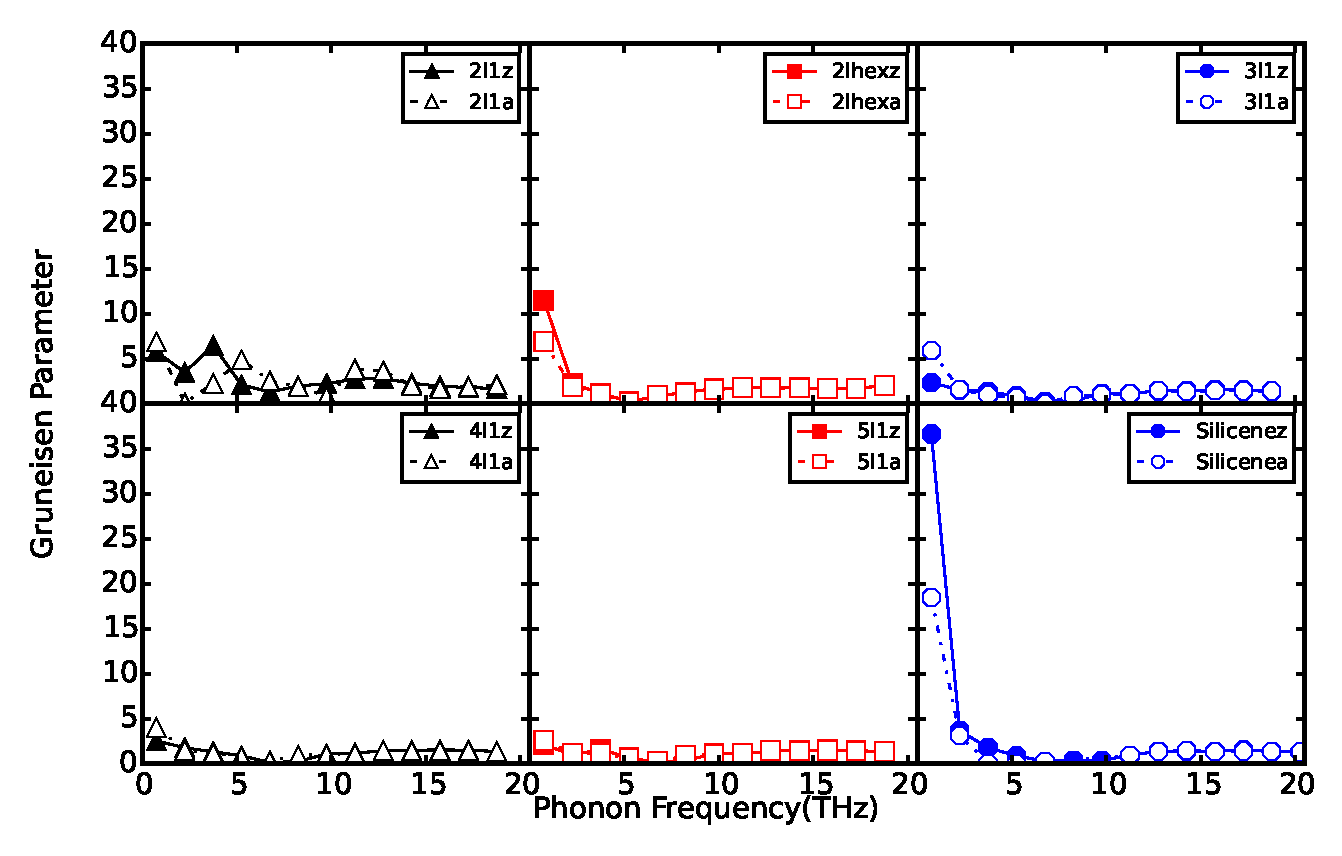
\includegraphics[width=0.48\textwidth]{images/gruneisen}
  \caption{\label{fig:gruneisen} (color online)Gruneisen parameters.}
\end{figure}

The anisotropy of phonon lifetime is due to the anisotropy of anharmonic effect. To quatitily check the anharmonic effect we calculate the Gruneisen parameters with 

\begin{equation}

\end{equation}

where V is the volumn of the unicell and $\omega$ is the phonon frequency. The shift of $\omega$ with V is due to the divirience from paraodic potential which reprensents for the harmonic situation. When the potenial is harmonic , all the Gruneisen parameters will vanish.
The Gruneisen parameters of all the structures are shown in FIG.\ref{fig:gruneisen}. The larger the anharmonic effect the smaller the scattering lifetime of the phonons. The most anharmonic phonons exist in the low frequency region and consist with previous result of phonon lifetime. The large difference between zigzag value and armchair could explain the anisotropy of phonon scattering. 

To obtain a clear connection between  the surface characteristic we also statistic the force constants of different position of the structures. 



\section{CONCLUSIONS}

By means of non-equilibrium molecular dynamics simulation, we found that the thermal transport properties of multilayer silicon structures have significant surface effect and size effect in thickness direction. Under the influence of double layer surface reconstruction, the thermal conductivity of the bilayer silicon can reach up to 11.6 W/mK (2l1 structure), and can be as low as 1.2 W/mK (2l2 structure) and the anisotropy can be as high as 57.3\%. The smooth surface is favorable for heat conduction, while the rough surface can greatly suppress the heat conduction. The ultra-low thermal conductivity indicates that the bilayer silicon has good thermoelectric properties. In the 3-6 layer multilayer silicon with the same $2 \times 1$ surface reconstruction the zigzag direction is more heat conducive. With the increase of the number of layers, the thermal conductivity of the zigzag direction changed little, but the thermal conductivity increased significantly in the armchair direction, and the anisotropy of thermal conductivity decreased. The thermal conductivity anisotropy of the multilayer silicon with 10 layers is very small, which is consistent with the bulk Si and monolayer silicene. This work could be helpful in the field of heat management, thermoelectric applications involving silicon and other multilayer nano materials in the future.

\quad \\
\section{ACKNOWLEGEMENTS}
This paper was partially supported by the National Natural Science Foundation of China, the Special Funds for Major State Basic Research, the Foundation for the Author of National Excellent Doctoral Dissertation of China, the Program for Professor of Special Appointment at Shanghai Institutions of Higher Learning, and the Research Program of Shanghai Municipality and the Ministry of Education.


\bibliography{ref}
\end{document}
